
\section{Arquitecturas de Servicios de Transferencia de Estado Representacional}
\label{\detokenize{chapter_one/rest:arquitecturas-de-servicios-de-transferencia-de-estado-representacional}}\label{\detokenize{chapter_one/rest::doc}}

\subsection{Protocolo de Transferencia de Hipertexto}
\label{\detokenize{chapter_one/rest:protocolo-de-transferencia-de-hipertexto}}
\begin{remark}
El Protocolo de Transferencia de Hipertexto o HTTP (por sus siglas en inglés)
es un protocolo de la capa de aplicación para sistemas de información
hipermedia distribuidos y colaborativos.

\end{remark}

Los navegadores web, servidores y todas las aplicaciones web
relacionadas se comunican entre ellas a través de este protocolo. Es la
base de la World Wide Web. Cada vez que se realiza una transacción en la
web, HTTP es invocado.

El contenido de la Web reside en servidores web. Los servidores web
“hablan” el protocolo HTTP, por lo que son llamados servidores HTTP.
Estos servidores HTTP almacenan datos de internet y proveen estos datos
cuando son solicitados por los clientes HTTP. Los clientes hacen
peticiones HTTP a los servidores, y los servidores regresan los datos
solicitados en respuestas HTTP. Juntos, los clientes y servidores HTTP
conforman los componentes básicos de la World Wide Web.

Los servidores web organizan y almacenan los \sphinxstyleemphasis{recursos web}. Un recurso
web es la fuente del contenido web. La forma más simple de un recurso
web es un archivo estático en el sistema de archivos del servidor web.
Estos archivos pueden contener cualquier cosa: archivos de texto,
imágenes en formato JPEG, archivos de video MP4, etcétera. Sin embargo,
los recursos no son necesariamente archivos estáticos. Pueden ser
programas que generen contenido cuando se les solicite. Estos recursos
dinámicos pueden generar contenido de acuerdo a la identidad de un
usuario, hora del día, etc. Estos te pueden mostrar imágenes en vivo de
una cámara, acciones, o hacer búsquedas en bases de datos.
En resumen, un recurso es cualquier tipo de fuente de contenido.

Una \sphinxstyleemphasis{transacción} en HTTP consiste de un comando de \sphinxstyleemphasis{solicitud} o \sphinxstyleemphasis{petición} (enviada
desde un cliente a un servidor), y una \sphinxstyleemphasis{respuesta} como resultado (enviado
del servidor al cliente). Esta comunicación se lleva a cabo con bloques
de datos, con un formato definido, llamados \sphinxstyleemphasis{mensajes} HTTP.


\subsubsection{Métodos}
\label{\detokenize{chapter_one/rest:metodos}}
El protocolo HTTP soporta varias peticiones diferentes,
conocidas como métodos HTTP. Cada mensaje de solicitud HTTP tiene un
método. El método le dice al servidor que acción realizar (buscar una
página web, eliminar un archivo, etc.). Los cuatro métodos más usados
son:
\begin{description}
\item[{GET.}] \leavevmode
Obtiene una representación del recurso. El cliente envía una
solicitud GET para pedir la representación de un recurso,
identificado por un URL.

\item[{DELETE.}] \leavevmode
Destruye el recurso. El cliente envía un DELETE cuando desea que un
recurso desaparezca.

\item[{POST.}] \leavevmode
El método POST tiene dos trabajos. El primero es POST-to-append, en
el cual, cuando se envía un POST-to-append a un recurso, se crea un
nuevo recurso debajo de este. Cuando un cliente envía una petición
POST-to-append, este envía una representación del recurso que quiere
crear en el cuerpo de la petición.

El otro trabajo de POST es llamado \sphinxstyleemphasis{overloaded} POST. La
especificación de HTTP dice que un POST puede ser usado para:
\sphinxstyleemphasis{Proveer un bloque de datos, desde el resultado de enviar un
formulario, hasta un proceso de manejo de datos}. El \sphinxstyleemphasis{proceso de
manejo de datos} puede ser cualquier cosa. Es “legal” enviar
cualquier dato como parte de la petición POST, para cualquier
propósito. La definición es tan vaga que una petición POST no tiene
una semántica de protocolo. En pocas palabras POST no significa
“crear un nuevo recurso” significa cualquier cosa. Usar un POST para
realizar un PUT, DELETE, PATCH, etc., es un overloaded POST.

\item[{PUT.}] \leavevmode
Reemplaza el estado del recurso con uno dado en la representación.
Una petición PUT, es una solicitud para modificar el estado de un
recurso. El cliente toma la representación obtenida de GET, la
modifica, y envía de regreso dentro de la petición PUT.

\end{description}

Existe otro método que no está definido en el estándar HTTP pero sí en
el apéndice RFC 5789:
\begin{description}
\item[{PATCH.}] \leavevmode
Modifica parte de el estado del recurso basado en una representación
dada. Si algún pedazo del estado del recurso no es mencionando en la
representación, lo deja como está. PATCH es como PUT pero permite
pequeños cambios en el estado del recurso.

\end{description}


\subsubsection{Status codes}
\label{\detokenize{chapter_one/rest:status-codes}}
Todo mensaje de respuesta HTTP trae consigo un código de estado. El
código de estado es un código de tres dígitos que le dice al cliente si
la petición fue exitosa o si otras acciones son requeridas. En la
tabla \ref{\detokenize{chapter_one/rest:table-status-code}} se muestran algunas categorías
de los códigos de estado más comunes.


\begin{savenotes}\sphinxattablestart
\centering
\sphinxcapstartof{table}
\caption{Categorías de los códigos de estado. \label{\detokenize{chapter_one/rest:table-status-code}}}
\sphinxaftercaption
\begin{tabulary}{\linewidth}[t]{|T|T|}
\hline
\sphinxstylethead{ 
Categoría
\unskip}\relax &\sphinxstylethead{ 
Descripción
\unskip}\relax \\
\hline
1xx: Informativo
&
Esta clase de códigos indican una respuesta provisional.
\\
\hline
2xx: Éxito
&
Indican que la petición del cliente fu aceptada exitosamente.
\\
\hline
3xx: Redirección
&
Indica que el cliente debe realizar acciones adicionales para completar la petición.
\\
\hline
4xx: Error del cliente
&
Esta categoría es para casos en las que el cliente parece haberse equivocado.
\\
\hline
5xx: Error del servidor
&
El servidor tomar responsabilidad del error.
\\
\hline
\end{tabulary}
\par
\sphinxattableend\end{savenotes}


\subsubsection{Mensajes}
\label{\detokenize{chapter_one/rest:mensajes}}
Los mensajes HTTP son secuencias de caracteres simples. Debido a que son
texto plano, y no binarios, son fáciles de leer y escribir por humanos.
Se llaman mensajes de petición si son enviados desde algún cliente web a
un servidor web. Los mensajes de los servidores a los clientes se
conocen como mensajes de respuesta.

Un mensaje HTTP consiste de tres partes:
\begin{description}
\item[{Línea inicial.}] \leavevmode
Indica qué hacer cuando se realiza una petición o qué sucede cuando
se envía una respuesta.

\item[{Campos del encabezado.}] \leavevmode
Cero o más campos de encabezado siguen después de la línea inicial.
Cada campo consiste de un nombre y un valor, separado por un punto y
coma. Los encabezados terminan con un espacio en blanco.

\item[{Cuerpo.}] \leavevmode
Después del espacio en blanco sigue un cuerpo del mensaje opcional
que contiene cualquier tipo de datos. El cuerpo de la petición
lleva datos al servidor web; el cuerpo de la respuesta carga
datos de regreso al cliente. A diferencia de la línea inicial y los
encabezados, el cuerpo puede contener datos binarios arbitrarios
(imágenes, videos, audio, aplicaciones, etc.).

\begin{figure}
    \centering
    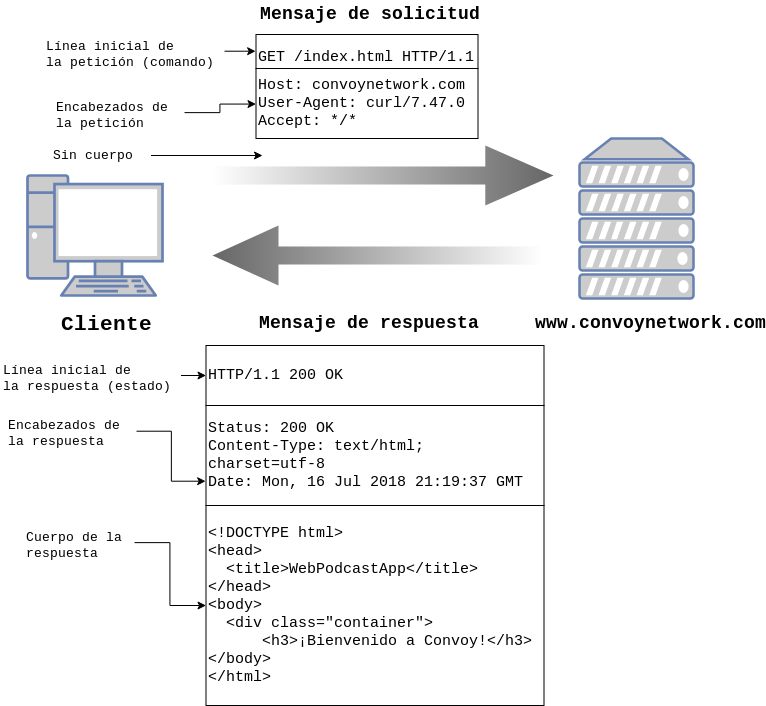
\includegraphics[scale=0.5]{figures/http_message.png}
    \caption{Ejemplo de la estructura de un mensaje de solicitud y de respuesta. El cliente solicita el archivo \texttt{index.html} mediante
    un \texttt{GET} y el servidor le regresa el archivo con un código de estado
    200.}
    \label{http-message}
\end{figure}

\end{description}


\subsection{World Wide Web}
\label{\detokenize{chapter_one/rest:world-wide-web}}
La World Wide Web o Web (Red Informática Mundial en español)  es un espacio de
información en el cual los objetos de interés, conocidos como \textit{recursos},
son identificados por Identificadores de Recursos Uniformes (URI por sus
siglas en inglés). En diciembre de 1990, Tim Bernes-Lee comenzó este proyecto,
donde inventó e implementó, entre otras cosas:
\begin{itemize}
\item {} 
El Identificador de Recursos Uniforme, una sintaxis que asigna a cada documento web una dirección única.

\item {} 
El Protocolo de Transferencia de Hipertexto (HTTP), un lenguaje basado en mensajes que las computadoras pueden usar para comunicarse a través de internet.

\item {} 
El Lenguaje de Marcas de Hipertexto (HTML), para representar documentos informativos que contienen enlaces a documentos relacionados.

\item {} 
El primer servidor web.

\item {} 
El primer navegador web, llamado «Nexus».

\end{itemize}

Desde el momento que el proyecto se publicó, comenzó a crecer exponencialmente.
El tráfico de la web estaba superando la capacidad de la infraestructura del internet.


\subsubsection{Arquitectura web}
\label{\detokenize{chapter_one/rest:arquitectura-web}}
A finales de 1993, Roy Fielding, a través de un análisis, reconoció que la escalabilidad
de la web estaba gobernada por un conjunto de restricciones clave.
Fielding agrupó en seis categorías esas restricciones y de manera manera colectiva
se refirió a ellas como el \sphinxstyleemphasis{estilo arquitectónico de la web}. Las
restricciones se describen a continuación.


\paragraph{Cliente servidor}
\label{\detokenize{chapter_one/rest:cliente-servidor}}
La web es un sistema basado en la dupla cliente-servidor, en la cual clientes y servidores
tienen distintos papeles. Estos pueden ser implementados y desarrollados independientemente,
usando cualquier lenguaje o tecnología, con tal que de que se ajusten a la \sphinxstyleemphasis{interfaz uniforme de la web}.


\paragraph{Interfaz uniforme}
\label{\detokenize{chapter_one/rest:interfaz-uniforme}}
Las interacciones entre los componentes web (clientes, servidores e intermediarios),
dependen de la uniformidad en sus interfaces. Si cualesquiera de estos componentes se
salen de los estándares establecidos, entonces la comunicación en la web
se rompe.

Los componentes web interactúan consistentemente dentro las siguientes
cuatro restricciones de la interfaz uniforme.

\begin{itemize}
    \item 
    Identificación de recursos:
Como se mencionó anteriormente, los elementos dentro de la web son
conocidos como \sphinxstyleemphasis{recursos} y tienen un identificador único. Por ejemplo, una
página web como \sphinxstyleemphasis{http://convoynetwork.com/}, identifica de manera única el
recurso en la raíz del sitio web.


\item Manipulación de recursos a través de sus representaciones:
Los clientes manipulan representaciones de recursos. Un mismo
recurso puede ser representado de diferentes formas a diferentes
clientes. Por ejemplo, un documentos puede representarse como un HTML
para un navegador web, y un JSON para un programa automatizado. La idea
principal es que la representación es una manera de interactuar con el recurso
pero no es el recurso en sí.


\item Mensajes autodescriptivos:
El estado deseado de un recurso puede ser representado dentro del mensaje
de petición del cliente. El estado actual de un recurso puede estar representado
dentro del mensaje de respuesta por parte del servidor.
Los mensajes autodescriptivos pueden incluir metadatos para comunicar
detalles adicionales con respecto al estado del recurso, el formato
de representación y tamaño, y el mensaje mismo.
Un mensaje HTTP provee \sphinxstyleemphasis{encabezados} para organizar varios tipos de
de metadatos en campos uniformes.


\item Hipermedia como el motor del estado de la aplicación (HATEOAS):
La representación del estado de un recurso incluye enlaces a recursos
relacionados. Los enlaces son los hilos que entrelazan la web, permitiendo
a los usuarios moverse a través de aplicaciones y datos de una manera directa
y significativa. La presencia, o ausencia, de un enlace en una página es una
parte importante del estado del recurso actual.


\end{itemize}

\paragraph{Sistema de capas}
\label{\detokenize{chapter_one/rest:sistema-de-capas}}
Las restricciones del sistema en capas permiten que intermediarios de red como
los proxies y puertas de acceso sean desplegadas de manera transparente entre el cliente
y el servidor usando una interfaz uniforme de la web. Intermediarios basados
en la red se usan para reforzar la seguridad, almacenamiento en caché de
respuestas, y balanceo de carga.


\paragraph{Caché}
\label{\detokenize{chapter_one/rest:cache}}
El almacenamiento en caché es una de las restricciones más importantes de la
arquitectura de la web. Las restricciones de la caché dan órdenes a un servidor
web para declarar la \sphinxstyleemphasis{cacheabilidad} de cada datos de la respuesta.
Guardar en la caché datos de la respuesta pueden ayudar a reducir
la latencia percibida por el cliente, aumentar la disponibilidad
general y confiabilidad de una aplicación, y controlar la carga
de un servidor web. En resumen, el almacenamiento en caché
reduce el \sphinxstyleemphasis{costo} general de la Web.


\paragraph{Stateless}
\label{\detokenize{chapter_one/rest:stateless}}
La restricción stateless dicta que un servidor web no está obligado
a memorizar el estado de sus aplicaciones cliente. Como resultado,
cada cliente debe incluir toda la información contextual que considere
sea relevante en cada interacción con el servidor web. Los servidores
web solicitan a los clientes administrar la complejidad de comunicar
el estado de su aplicación tal que el servidor web puede servir a un número
mayor de clientes.


\paragraph{Código bajo demanda}
\label{\detokenize{chapter_one/rest:codigo-bajo-demanda}}
Esta restricción permite a los servidores web transferir temporalmente
programas ejecutables, tales como scripts o extensiones a los cliente.
El código bajo demanda tiende a establecer un acoplamiento de tecnología
entre servidores web y sus clientes, ya que el cliente debe tener la habilidad
de entender y ejecutar el código que descarga cuando lo desea desde el servidor.
Por esta razón, el código bajo demanda es la única restricción del
estilo arquitectónico de la web que se considera opcional.


\subsection{Transferencia de Estado Representacional (REST)}
\label{\detokenize{chapter_one/rest:transferencia-de-estado-representacional-rest}}
En el año 2000, después de que la crisis de la escalabilidad de la web se
evitó, Fielding llamó y describió al estilo arquitectónico de la web en su
trabajo doctoral. \sphinxstylestrong{Transferencia de Estado Representacional} (REST por
sus siglas en inglés) fue el nombre que Fielding dio a su descripción del
estilo arquitectónico de la web, que está compuesto por las restricciones
mencionadas previamente.

La Transferencia de Estado Representacional es un estilo de arquitectura de software.
Este estilo es
una abstracción de elementos arquitectónicos dentro de un sistema de hipermedia
distribuido como es la Web. REST ignora los detalles de la implementación de
componentes y sintaxis de protocolos de manera que pueda enfocarse en los
papeles de los componentes, las restricciones sobre su interacción con otros
componentes, y la interpretación de elementos de datos significativos.
Abarca las limitaciones fundamentales sobre los componentes, conectores y datos
que definen las bases de la arquitectura web y, por lo tanto, la esencia de su
comportamiento como una aplicación basada en red. REST no es un estándar, sin
embargo sí un conjunto de restricciones. No está atado al protocolo HTTP,
pero a menudo se asocia con éste.


\subsubsection{API REST}
\label{\detokenize{chapter_one/rest:api-rest}}
Un \sphinxstyleemphasis{servicio web} es un sistema de software diseñado para admitir
la interacción interoperable de una máquina a otra  máquina a través de una red.
Programas cliente usan \sphinxstyleemphasis{interfaces de programación de aplicaciones} (API
por sus siglas en inglés) para comunicarse con servicios web. Generalmente
hablando, una API expone un conjunto de datos y funciones para facilitar
interacciones entre programas de computadora y permitiendo que
intercambien información.

\begin{figure}[htbp]
\centering
\capstart

\noindent\sphinxincludegraphics[scale=0.60]{{web_service_cycle}.png}
\caption{Una API web es el frente de un servicio web, escuchando y respondiendo las peticiones de los cliente directamente.}\label{\detokenize{chapter_one/rest:web-service-cycle}}\end{figure}

El estilo arquitectónico REST se aplica comúnmente al diseño de API para
servicios web modernos. Una API web que sigue el estilo REST es una API REST.
Tener una API REST hace a un servicio web RESTful. Una API REST está formada de
recursos entrelazados.\\

\begin{remark}
REST es una arquitectura basada en recursos. Se accede a un recurso a través
de una interfaz común basada en los métodos estándar de HTTP. REST
solicita a los desarrolladores usar métodos HTTP explícitamente
y de una forma que sea consistente con la definición del protocolo.
Cada recurso se identifica con un URL. Todos los recursos deben soportar
las operaciones HTTP más comunes, además REST permite que ese recurso
tenga diferentes representaciones, por ejemplo, texto, XML, JSON, etc.
El cliente REST puede solicitar una representación en específico por
medio del protocolo HTTP. La \hyperref[\detokenize{chapter_one/rest:rest-struct}]{Tabla \ref{\detokenize{chapter_one/rest:rest-struct}}} describe
los elementos usados en REST.
\end{remark}


\begin{savenotes}\sphinxattablestart
\centering
\sphinxcapstartof{table}
\sphinxcaption{Elementos de REST \label{\detokenize{chapter_one/rest:rest-struct}}}
\sphinxaftercaption
\begin{tabulary}{\linewidth}[t]{|T|T|}
\hline
\sphinxstylethead{ 
Elemento
\unskip}\relax &\sphinxstylethead{ 
Descripción
\unskip}\relax \\
\hline
Recurso
&
Objetivo conceptual de una referencia de hipertexto. Por ejemplo: podcast.
\\
\hline
Identificador de recurso
&
Un URL que identifica un recurso en específico. Por ejemplo: \sphinxurl{http://convoynetwork.com/podcast/123}
\\
\hline
Metadatos del recurso
&
Información que describe al recurso. Por ejemplo: autor, etiqueta, etc.
\\
\hline
Representación
&
El contenido del recurso. Por ejemplo: un JSON, un HTML o una imagen JPEG.
\\
\hline
Metadatos de la representación
&
Información que describe como procesar la representación. Por ejemplo: tipo de medio, fecha, etc.
\\
\hline
Datos de control
&
Información que describe cómo optimizar el procesamiento de respuesta. Por ejemplo: if-modified-since, cache-control-expiry.
\\
\hline
\end{tabulary}
\par
\sphinxattableend\end{savenotes}

